% Created 2021-08-10 Tue 13:32
% Intended LaTeX compiler: pdflatex
\documentclass[12pt,spanish,oneside,breaklinks]{book}
\usepackage[utf8]{inputenc}
\usepackage[T1]{fontenc}
\usepackage{graphicx}
\usepackage{grffile}
\usepackage{longtable}
\usepackage{wrapfig}
\usepackage{rotating}
\usepackage[normalem]{ulem}
\usepackage{amsmath}
\usepackage{textcomp}
\usepackage{amssymb}
\usepackage{capt-of}
\usepackage{hyperref}

\parskip=10pt
\parindent=0in
\usepackage[spanish, mexico]{babel}
\usepackage{url}
\usepackage{appendix}
\usepackage{rotating}
\usepackage{url}
\def\UrlBreaks{\do\/\do-}
\usepackage{breakurl}
%\usepackage[breaklinks]{hyperref}
\begin{document}

\newpage

\newpage

\thispagestyle{empty}

\setcounter{page}{1}
\begin{center}
\begin{tabular}{c}
\hline
 \large \emph{\textsc{Instituto Tecnológico Autónomo de México}} \\

\hline
\end{tabular}

\vspace{10pt}

\centering

\includegraphics[width=0.8\linewidth]{img/Logo_ITAM.jpeg}

\vspace{20pt}


\Large Mapeo en Respuesta a Emergencias: Caso \texttt{\#Verificado19s}



\vspace{30pt}

\normalsize Caso

\vspace{12pt}

que para obtener el grado de

\vspace{12pt}

Maestro en Ciencia de Datos

\vspace{12pt}

presenta

\vspace{12pt}

Miguel Angel Escalante Serrato

\vspace{32pt}

\begin{tabular}{lcr}
Ciudad de México. & \hspace{80pt} & 2021
\end{tabular}

\end{center}


\newpage
\setcounter{page}{1}
\pagenumbering{roman}
\mbox{ }
\vspace{80pt}
\mbox{ }

Con fundamento en los artículos 21 y 27 de la Ley Federal del Derecho de Autor y como titular de los derechos moral y patrimonial de la obtra titulada ``\textbf{Mapeo en Respuesta a Emergencias: Caso \texttt{\#Verificado19s}.}'', otorgo de manera gratuita y permanente al Instituto Tecnológico Autónomo de México y a la Biblioteca Raúl Bailléres Jr., autorización para que fijen la obra en cualquier medio, incluido el electrónico, y la divulguen entre sus usuarios, profesores, estudiantes o terceras personas, sin que pueda percibir por tal divulgación una contraprestación.
\vspace{20pt}
\begin{center}
\textbf{Miguel Angel Escalante Serrato}
\vspace{80pt}

\begin{tabular}{p{2cm}cp{2cm}}

\hline \\


&Fecha & \\
\\
\\
\\
\\
\\
\\
\\
\\
\hline \\

 & Firma &

\end{tabular}
\end{center}



\newpage
\thispagestyle{empty}

\begin{center}

\vspace{40pt}
\[\]
\[\]
\[\]
\begin{tabular}{c}
\hline
 \\[.2cm]
\Huge
\textbf{Mapeo en Respuesta a Emergencias:  }\\
\Huge\textbf{Caso \texttt{\#Verificado19s}}\\[14pt]
\normalsize
Miguel Angel Escalante Serrato \\[.2cm]

\hline
\end{tabular}
\end{center}



\newpage
\vspace*{\fill}
\begin{flushright}
A mi familia, que sin ellos nada de esto sería posible.
\vfill
\end{flushright}
\newpage
\mbox{ }
\vspace{80pt}
\begin{flushright}
\textsc{\large Agradecimientos} \\
\vspace{12pt}
A mis padres ya que de ellos aprendo los fundamentos para enfrentar esto y todos los retos de la vida.

A Alfredo Garbuno que tuvo un impacto particular en la escritura de este documento.

A Andrea García Tapia, ya que gracias a ella comenzó el esfuerzo real de documentar este esfuerzo.

A mis sinodales Beatriz Rumbos y Fernando Esponda, por sus prontos y atinados comentarios.

A mis amigos y mi red de soporte, Irving, Paris, Nivi, Nano, Andy, Animalito, Fer.

A Luly por su apoyo, cariño y empuje con este proceso.

\end{flushright}
\newpage


\frontmatter

\tableofcontents

\mainmatter

\chapter{Introducción}
\label{sec:org504c50c}

El 19 de septiembre de 2017 se suscitó un sismo de magnitud 7,1 grados en la escala Richter \cite{cnn}, que si bien fue menor al sismo suscitado unos días antes en la Ciudad de México\footnote{El 7 de septiembre con magnitud 8,1 en la escala Richter.}, tuvo repercusiones que se hicieron inmediatamente presentes.

Los daños generados en toda la ciudad fueron importantes, con edificios afectados en las delegaciones Cuauhtémoc, Benito Juárez, Tlalpan, Iztapalapa, Xochimilco y Coyoacán \cite{ap19s}; esto sin tomar en cuenta las afectaciones  generadas en las entidades aledañas a la Ciudad de México. Los daños abarcaron desde pequeñas afectaciones a los edificios, hasta derrumbes de unidades habitacionales completas.

Dada la densidad poblacional de la zona, y el rango de afectaciones que se presentaron, fue difícil hacer una primer evaluación de lo ocurrido. Las redes telefónicas y de transporte, colapsaron por el incremento repentino de la demanda \cite{telcom19s}. Los ciudadanos tenían total incertidumbre, no había manera de ver si sus hogares aún estaban de pie, ni tampoco de si sus seres queridos estarían bien. La falta de información y la impotencia fueron un factor importante en cómo se vivieron las siguientes horas. La mayor parte de la población regresó a sus respectivos hogares. Ya fuera en auto, motocicleta, bicicleta o caminando, todos regresaron a sus casas. Poco a poco las diferentes redes fueron aliviando, los bloqueos informáticos cesaron y fue regresando la luz y el internet a las personas \cite{ift}.

\section{Captura de información}
\label{sec:org8aaf370}

Por medio de dispositivos móviles, la mayor parte de la población tiene en sus bolsillos herramientas para grabar y transmitir videos en tiempo real. Por supuesto, en aquel momento el problema principal fue la falta de red telefónica para transmitirlos. Conforme avanzaba el día había periodos en los que se podía percibir señal que facilitaba el flujo de mensajes. Mismos que llegaban por medio de grupos de \emph{Whatsapp}. La información estaba fragmentada. Había videos alarmantes de diferentes situaciones: personas evacuando edificios con un paneo\footnote{Vistazo previo que se hace con una cámara sobre algo antes de fijar el objetivo.} de la ciudad envuelta en  humo y polvo; tanques estacionarios explotando; edificios derrumbándose. La generación de información fue inmediata y en grandes cantidades.


El problema principal con tal generación de información es que no tenía ningún orden. Se compartían mensajes reenviados vía \emph{WhatsApp}, publicaciones en \emph{Facebook} e \emph{Instagram}. Todos sin ninguna información adicional de lo que estaba pasando. La  atención se concentró en los videos más escandalosos\footnote{Una búsqueda realizada por el término =video sismo 19 de septiembre= arroja resultados con alrededor un millón y medio de visualizaciones por resultado.}. Ante este problema Sergio Beltrán arquitecto de profesión quien utilizaba mapeos de la ciudad para su trabajo, tuvo la idea de utilizar MyMaps de Google\cite{mymap} para comenzar a puntear la información recibida en un mapa público.

Al publicar el mapa, varios ex-compañeros de Beltrán se ofrecieron como voluntarios para seguir agregando información. Conforme la red de colaboradores y usuarios creció, también lo hizo la carga que tuvo la plataforma para mantener activo el mapa. El 19 de septiembre el sitió recibió alrededor de un millón de visitas. El problema fue que en la madrugada del 20 de septiembre el mapa dejó de funcionar. No se podía editar más. Sin embargo,  aún se podía ver la información pero ya no era posible actualizar el mapa.

\section{Grupos emergentes auto-organizados}
\label{sec:org2f13d98}

Ante eventos de esta magnitud, la efectividad de la respuesta a la emergencia, depende en parte, de la velocidad y magnitud de la misma. Una respuesta muy fuerte ante desastres puede salvar muchas vidas; sin embargo hay recursos limitados dentro del gobierno. Los actores gubernamentales no pueden ayudar a todas las personas que lo requieren en el momento adecuado \cite{flood}.

Los desastres estimulan respuestas espontáneas (que anteceden a la mobilización de organizaciones formales), a través de grupos voluntarios auto-organizados, conformados por individuos dentro y fuera de las comunidades afectadas por el desastre. Estos grupos espontáneos y "emergentes"  son una característica común de los desastres  \cite{emergentgroups}. La respuesta de los actores gubernamentales es de muchas maneras desconectada e impredecible. Muchas líneas de comunicación están poco articuladas y la información llega con diferentes niveles de detalle y precisión\cite{coord}.

El voluntariado, a través de individuos y grupos emergentes, es un recurso importante para la respuesta ante la emergencia. Es muy probable que dado el crecimiento de los centros urbanos, aunado al incremento en la densidad  y proximidad de poblaciones urbanas, este cobre una mayor importancia. La población local es fundamental para la respuesta ante los desastres \cite{coord}.

Durante la respuesta al sismo del 19 de septiembre del 2017, uno de estos grupos emergentes auto-organizados nació y se consolidó como \texttt{\#Verificado19s}, dentro de este colectivo tuve la fortuna de liderear al equipo técnico y tecnológico del colectivo. En ese momento coordinaba un equipo de más de 10 personas en la empresa donde laboraba, mismas que se volvieron la espina dorsal de la implementación de los procesos automatizados. Llegando a coordinar a un equipo de más de 40 personas en sitio, fue uno de los esfuerzos más gratificantes que he lidereado, el privilegio de coordinar a tantas personas tan talentosas y con un objetivo tan claro, es algo que difícilmente se olvida.

\section{Mapeo de información}
\label{sec:org748f04e}

Empatar las necesidades de ayuda y los esfuerzos de rescate a tiempo de manera efectiva es uno de los retos más importantes de la respuesta humanitaria. Gobiernos y organizaciones humanitarias tienen una demanda explicita de información relevante, accionable y encontrrable. Sin embargo, la información es de los recursos más perecederos\cite{bigdatahum}, ya que la información deja de ser relevante, muchas veces, antes de haberse tomado alguna acción. De hecho, lo que usualmente consideramos como "rápido" es lento: los medios de información usualmente son acusados de sensacionalismo en las crísis y también de reportar información falsa, fuera de tiempo y repetitiva. Los reporteros tienden a ser ajenos a las comunidades locales y sus condiciones \cite{networkshum}.

Se puede definir un mapa comunitario como un conjunto de servicios via un proveedor internacional y/o una comunidad en línea que recolecta, analisa y mapea información crítica alrededor de poblaciones que fueron afectadas por algún desastre. \cite{crowdsourced} Dentro del sector humanitario el mapeo comunitario ha revolucionado la manera en que se percibe la respuesta a la crísis, en concreto, gracias a la habilitación de las comunidades afectadas por algún desastre para definir la manera en la que reciben ayuda \cite{harvardhuman}.

Se han discutido las virtudes y limitaciones de mapas comunitarios para su uso en projectos no-gubernamentales y humanitarios. Sin embargo, el terremoto del 2010 en Haití,  trajo al frente el proceso de mapeo comunitario de crisis. Durante y después del sismo la población de Haití hacía pedidos de ayuda usando redes sociales y tecnologías móbiles, este esfuerzo fue coordinado por \textit{Humanitarian Open Street Map} y \textit{Ushahidi} usando \textit{OpenStreetMap} \cite{crowdsourced}.

\newpage
\chapter{Problema}
\label{sec:org7ca56db}

El mapa tenía como entrada capturas manuales de diferentes amigos y conocidos de Sergio Beltrán.  Conforme la cantidad de información recabada fue creciendo, la confianza general aumento. Y con esto, más personas aportaron al mapeo de los diferentes puntos. El crecimiento del número de usuarios al agregar puntos de información de manera desorganizada eventualmente rebasó la capacidad de la herramienta. El mapa dejó de permitir nuevas cargas de información. Esto se explica porque la herramienta de la plataform de Google,  MyMaps, está diseñada para uso personal.

Ante tal situación y aunado a las peticiones de información y recursos que llegaban al colectivo, los voluntarios tomaron por iniciativa capturar lo que llegaba en papel. Esto hizo problemático el manejo de todas las capturas que se seguían recabando, ya que posteriormente a escribirlos en papel, había que encontrar la manera de digitalizarlos. Todo esto para poder compartir la información. 

El objetivo principal fue encontrar una manera de capturar todos los puntos de información que llegaran al colectivo, digitalizarlos y volverlos disponibles a diferentes actores. Se propuso implementar una automatización de la ingesta de datos, para luego publicarla en el mapa previamente mencionado, de tal forma que hubiera una fuente de información con todo lo recabado y lo que se estaba por recabar. Una de las decisiones tomadas fue el  tomar en cuenta todas las fuentes confiables de información\footnote{Con esto nos referimos a fuentes de información con instituciones respaldándolas.} que se encontraran para agregar a las sábanas de información del mapa.

Al momento de comenzar la colaboración se tuvieron que resolver diferentes temas, en concreto:

\begin{enumerate}
\item Sobrecarga del mapa
\item Ingesta de información.
\item Unificación entrada de información
\item Unificación de salida de información.
\end{enumerate}

Uno de las principales problemas enfrentados conforme fue creciendo el movimiento, fue el hecho de que la población no tiene el entrenamiento para reportar incidentes o puntos de información. Por lo que se encontraron una serie de puntos de información falsos. Estos eventos se verificaron como falsos al momento de atender los  reportes y encontrar que no existía tal problema. Al automatizar la entrada de información, estos puntos tenían el riesgo de aumentar considerablemente.

El mecanismo pensado para verificar la información reportada por los ciudadanos fue el generar una capa de verificación humana. Esto es, para cada punto reportado, un voluntario del colectivo se aproximaba al lugar para verificar que el hecho efectivamente estuviera ocurriendo. Con ello, se generó una fuente de información mucho más confiable que los reportes en bruto de todos los ciudadanos.

Uno de las principales problemáticas enfrentadas conforme fue creciendo el movimiento, fue el hecho que la población no tiene el entrenamiento para reportar incidentes o puntos de información, se vuelve evidente tras encontrar diversos reportes falsos; se verificaron como falsos al atender el problema reportado para encontrar que no existía tal problema. Al automatizar la cantidad entradas reportadas, estos puntos tenían el riesgo de aumentar bastante.

El mecanismo pensado para verificar la información reportada por los ciudadanos fue el generar una capa de verificación humana, esto es, para cada punto reportado, un voluntario del colectivo se aproximaba al lugar para verificar que el hecho genuinamente estuviera ocurriendo. Con ello, se generó una fuente de información mucho más confiable que los reportes en bruto de todos los ciudadanos.

\newpage

\chapter{Solución implementada}
\label{sec:orgca60366}

Para enumerar las distintas soluciones que se implementaron durante este ejercicio, hablaremos de los pasos del flujo de la información: \textbf{ingesta}, \textbf{procesamiento}, \textbf{inteligencia} y \textbf{visualización}.

\section{Ingesta}
\label{sec:orgfa5099b}

El primer punto a resolver dentro de todos los problemas que surgieron fue el migrar de las hojas de papel a un medio electrónico que pudiera ser escalable y fácil de distribuir.

\subsection{Formulario}
\label{sec:orgabe6006}

Lo primero que vino a la mesa, fue hacer una app (ya fuera móvil o para navegador) que conectara con una base de datos y pudiera hacer ediciones, verificaciones, agregar puntos de información. Sin embargo el problema fue la restricción de tiempo, además de que en ese momento los voluntarios con los que se contaba no tenían la experiencia necesaria como para desarrollar tal herramienta con la velocidad requerida.

Ante las limitantes de tiempo y buscando la flexibilidad para poder distribuir nuestro método de ingesta a una gran cantidad de personas, se buscó una herramienta que tuviera la capacidad de capturar el volumen necesario. Se tomó la decisión de usar Google Forms\footnote{https://www.google.com/forms/about/.}. Esta herramienta tiene todo lo necesario para hacer una ingesta rápida de información. Tiene campos de selección de opciones, texto libre, \emph{checkboxes}, carga de imágenes, etc. La información ingerida en estos formatos automáticamente se puede ver reflejada en una base de datos en Google Sheets\footnote{https://www.google.com/sheets/about/.}. La última, una plataforma que tiene la capacidad de guardar toda la información junto con la robustez de los servicios de Google en el formato de tabla (unidad de almacenamiento básica en un modelo relacional, \cite{codd}).

La información que inicialmente se pensaba recibir tenía que ver con los sitios de derrumbe para encontrar los distintos bienes que pudieran faltar o sobrar en cada uno de ellos. Inmediatamente surgió la necesidad de tener la ubicación de centros de acopio y albergues. Con ello nos dimos cuenta que teníamos que generar más de un flujo de ingesta de información. Se hicieron tres formularios para recibir información de sitios con daños, albergues y centros de acopio.

\subsection{Verificación de Información}
\label{sec:org77833d3}

La necesidad de verificar la información se hizo más evidente y lo que se implementó fue una capa de verificación intermedia. Gracias a todos los voluntarios, el foco que obtuvo la herramienta y el mapa que se viralizó, existían equipos grandes de voluntarios en distintas modalidades de transporte: a pie, en bicicleta o motocicleta.

Todos los voluntarios eran un par de ojos que ayudaban a visitar cada lugar reportado y verificar si el incidente fue verdadero. Con esto también surgió la necesidad de definir lo que significa que algo esté verificado. La definición que se acordó entre el equipo fue

\begin{quote}


Para que un evento esté verificado se requiere que se cumpla al menos una de las siguientes condiciones:

\begin{itemize}
\item El evento fue  visto con los ojos de la persona que reporta.
\item Al menos dos personas de confianza del reportante lo han presenciado.
\end{itemize}
\end{quote}

Desde el punto de vista de la información que llegaba, se dejaron los mismos formularios públicos, pero se agregaron otros tres formularios sólo para los verificadores. Los segundos formularios son los que finalmente se publicaban en el mapa y con los que el colectivo trabajó.

\subsection{Unificación}
\label{sec:org21dde91}

La última iteración de los formularios fue una unificación de los tres formatos en un punto de entrada.  El objetivo era aliviar la necesidad de tener tres diferentes enlaces para cada tipo de información. Esto incorporaba una capa adicional de complejidad y entablaba barreras para el flujo de la información. En el formulario unificado, se agregaron además otros dos tipos de puntos de información: transportes y voluntarios. Mismos que brindaron una mayor capacidad de proveer ayuda.

Los enlaces de los distintos formularios fueron publicados a través de redes sociales. En cuanto se tuvo una página web, los enlaces fueron migrados junto con instrucciones de cómo ser llenados con el objetivo de mayor claridad y tener un proceso de captura mas sencillo.

\section{Procesamiento}
\label{sec:org592dfbe}

La información que se obtuvo durante todo el tiempo que estuvo activo \texttt{\#Verificado19s}, era de naturaleza delicada, pues en la captura se incluyeron teléfono, nombre y ubicación de la persona que reportaba. Mismos que son privados y  no podían ser publicados en ningún momento.

\subsection{Ubicación}
\label{sec:org3479344}

Google Forms, fue una herramienta vital para la solución que se concretó. Sin embargo, tuvo ciertas limitantes en las entradas que podrían ser re-gistradas por los formularios. En particular, no se puede hacer la captura de la ubicación del teléfono con el que se está haciendo el formulario, esto añade un grado de complejidad no previsto y con alta probabilidad de error durante el proceso de captura.

La estimación de la ubicación se realizó a través de la interfaz de programación de aplicaciones (API, por sus siglas en inglés) de Google Maps\footnote{\url{https://www.google.com/maps/about/}.}. Se mandaba a ésta la dirección con atributos: calle, número, colonia y ciudad. La API respondía con las coordenadas estimadas para una dirección dada y con ello un punto geográfico que podíamos visualizar y registrar en un mapa.

Uno de los problemas con este acercamiento es que cuando la información estaba incompleta, la API daba coordenadas bastante lejanas al punto. Un ejemplo de esto es la calle de Escocia en la colonia Del Valle. En dicha dirección hubo dos derrumbes y cuando se reportó con la información incompleta, se recibieron de la API coordenadas en el país de Escocia.

Para eliminar el problema de los datos que la API identificaba fuera de las áreas demarcadas, aunado al corto tiempo que se tenía, se decidió eliminar los puntos lejanos a la Ciudad de México. El criterio fue utilizar la demarcación regional del resultado de la API. El mismo filtro fue aplicado cuando se incorporaron los reportes de los demás estados de la república. 

\subsection{Datos Personales}
\label{sec:org0178856}

Para poder publicar la información al mapa se requiere que no haya datos personales dentro de los puntos de información; en concreto, buscamos borrar el nombre y el teléfono de las personas que reportaron incidentes. Esto en conjunto con la geolocalización de las direcciones dió pie al primer proceso de extracción, transformación y carga (ETL, por sus siglas en el inglés) que se generó para \texttt{\#Verificado19s}.

En particular, se acordó que sólo los números telefónicos de los albergues y centros de acopio serían publicados. Sin embargo, aún hubo voluntarios que siguieron dando sus números personales. El problema fue que al ser publicada esta información se recibieron quejas inmediatas y se tuvieron que eliminar esas entradas de la base de datos.

Este último punto es uno de los puntos importantes a tomar en cuenta para futuras replicaciones en situaciones de emergencia. Es decir,  tomar todas las precauciones para que los datos de los voluntarios no sean expuestos, comprometiendo así tanto el crecimiento como la credibilidad del movimiento.

\subsection{Actualización}
\label{sec:org6103da2}

El fenómeno que se observó durante la respuesta al sismo evolucionó cada minuto. Por lo que tener un mecanismo de actualización de las distintas necesidades se volvió parte fundamental. Cada punto cambiaba dependiendo de nuevos descubrimientos o la llegada de recursos que fueron necesarios en alguna otra ubicación.

En particular, en redes sociales se encontró un problema fundamental con la publicación de las necesidades que se presentaron. Las publicaciones con fecha del 19 de septiembre seguían teniendo eco el 23 de septiembre. La falta de una hora y fecha de publicación entorpeció también la optimización de recursos.

Google Forms, a diferencia de una aplicación que permitiera manejo de información, no tiene manera de actualizar  entradas determinadas. Por lo que se tuvo que encontrar una manera de que esto se resolviera.

Se tomó la decisión de hacer actualizaciones de los distintos puntos con una nueva entrada en los formularios. Esto con el objetivo de que con cada actualización se llenara un  nuevo registro con la misma ubicación. La diferencia es que tenía  la información de las distintas necesidades de manera actualizada. Si se quería borrar algún punto, se tenía que mandar un formulario con las necesidades vacías y los mismos datos de ubicación.

El sistema de actualización planteado posee muchas fallas que son evidentes. Por ejemplo, era tedioso volver a escribir toda la información geográfica para actualizar los datos. Además, los errores de captura que se  podía cometer con la urgencia para los voluntarios eran abundantes. Esto generó problemas de punteo ya que todos los voluntarios fueron suceptibles a este fallo y la capa verificadora tampoco tenía un mecanismo para identificarlos.

Por otro lado, un problema adicional fue que distintos voluntarios reportaron el mismo sitio. Con la capa de verificación este problema fue mucho menor, ya que las necesidades más importantes venían de los verificadores cercanos.

Conforme pasó el tiempo, la información en el mapa dejó de ser relevante para efectos prácticos. Se decidió hacer un filtro temporal de un día a los puntos reportados. Lo que significa que  en cuanto se reportaba un incidente, se tenían que seguir haciendo reportes diarios para que los puntos no desaparecieran del mapa.

\section{Inteligencia}
\label{sec:org3fe1785}

Al final del día 20 de septiembre, ya se tenía una primera versión del ETL funcionando.  Se cargaba de forma manual al mapa final en MyMaps. Con la información que se iba recabando se tenía lo suficiente como para hacer una solución bastante robusta con el objetivo de parear la información de la oferta (recursos) con la de demanda (sitios necesitados).

El problema que apareció al tratar de hacer este modelo, es que no se tenía una manera fidedigna de tratar los sitios de desastre y centros de acopio como puntos de información editables de tal forma que pudieran ser actualizados o borrados. No se podía delimitar el sitio \(k\) y accionar con respecto a éste. Lo que sí se tenía era una serie de reportes con ligeros cambios en la dirección reportada. Además de las variaciones que había en dicho sitio.

Durante la madrugada del 21 de septiembre, una consultora se puso en contacto con el equipo. Ellos comentaron que el problema de unificar puntos y poder editarlos era análogo a una herramienta que tenían hecha para otro propósito. El compromiso fue que en cuestión de 12 horas, se podía adaptar su aplicación para que funcionara para las necesidades de \texttt{\#Verificado19s}. Conforme pasó el tiempo, fueron retrasando la entrega. Para el final del 24 de septiembre, aún quedó pendiente la entrega del compromiso que se tenía con \texttt{\#Verificado19s}.

En el momento se tomó la decisión de esperar esta herramienta para poder automatizar el pareo de oferta y demanda. Conforme pasó el tiempo esta necesidad se fue erosionando, ya que la optimización de los voluntarios fue más rápida y contundente ante las necesidades existentes.

\subsection{Coordinación Logística}
\label{sec:org60a454e}

Las voluntarias que estuvieron a cargo de unir las necesidades y los recursos (\emph{brokers}), fueron un equipo de 3 personas. Cada una de ellas, a través de grupos de confianza en \emph{WhatsApp} y \emph{Telegram}, se encargó de ir buscando para cada necesidad reportada alguien que pudiera suplir el material requerido.

En ese momento la organización humana se simplificó de tal forma que sólo había un encargado por sitio de derrumbe para reportar todo lo que se necesitaba al momento. Estas \emph{brokers} fueron centrales en el movimiento ya que gracias a ellas se agilizó bastante la velocidad con lo que se entregaron los materiales.

El problema de trabajar con recursos humanos son las necesidades fisiológicas como el descanso. Conforme pasaron las horas y eventualmente los días, este equipo se enfrentó con el cansancio y la falta de horas de sueño. Por un lado, se volvieron indispensables y, por otro, eso fue profundamente problemático tanto de manera interna como externa. El estrés al que este equipo estuvo sujeto era impresionante y eventualmente tuvieron que descansar. En este momento se volvió mucho más evidente la necesidad de generar un sistema robusto y redundante; ya sea con una herramienta automatizada o un equipo de personas que pudieran suplir a las personas dentro de las redes de confianza. Cuidar la salud tanto física como mental de los voluntarios es fundamental en un esfuerzo como \texttt{\#Verificado19s}.

\section{Visualización}
\label{sec:orgf9d31d7}

Todo el movimiento \texttt{\#Verificado19s} inició con un mapa y evolucionó a un sistema de gestión de recursos necesarios para el rescate de las víctimas de la crisis humanitaria que enfrentó México. El énfasis de haber utilizado una herramienta de visualización de esta naturaleza es que a pesar de la opinión que un mapa es una manera muy básica e incompleta de transmitir información, es una de las maneras más sencillas y claras para que la ciudadanía pueda acceder a ella en una situación de crisis.

\subsection{Diversidad de Fuentes}
\label{sec:org4ed6ab2}

En ese momento había distintos equipos capturando información de la misma índole que \texttt{\#Verificado19s}. Conforme se contactaron a estos equipos y brindaron el acceso a su base de datos, se tomó la decisión de publicar la información de todas las fuentes que estuvieran abiertas. Las primeras fuentes externas en cargarse fueron:
\begin{itemize}
\item Manos a la obra
\item Coordinación de Estrategia Digital Nacional
\item Descifra
\item Waze
\end{itemize}

La insistencia de tener todas las capas arriba fue para solidificar a \texttt{\#Verificado19s} como una plataforma unificadora y no sólo una más en respuesta al desastre. Todas las bases de datos que se recibieron se fueron añadiendo a los puntos del mapa original, sin embargo todo se tenía que unificar en una única capa. Cada punto en la capa se etiquetaba con el origen del dato y la información de cada punto.

El primer mapa, fue hecho y publicado en la plataforma MyMaps de Google. Tras la insistencia del equipo de Google a migrar a una plataforma más robusta, se tomó la decisión de hacer una migración al Google Crisis Map.

\section{Crisis Map}
\label{sec:orgc02fc55}

Google Crisis Map es una herramienta hecha para que los usuarios encuentren y usen información crítica durante una crisis. Esta herramienta, cuando se activa, es accesible desde Google Search y Google Maps. Al momento de atender el sismo de México en 2017, se pensó en un principio como una herramienta para visualizar datos relacionados a las crísis y respecto al clima. Sin embargo, el equipo de Google decidió desactivar el sitio de Google Crisis Map y el proyecto ha sido migrado al resto de los productos de Google \cite{googlecrisis}.

El equipo de Google fue muy insistente con el hecho de que la herramienta de Google Crisis Map, sería una opción mucho más robusta y resiliente a todo lo que se requería hacer. Las características principales que hicieron que se tomara la decisión de migrar a esa plataforma fueron: actualización de información más rápida y automática, posibilidad de conectar con Google Big Query, capas filtrables de información y escalabilidad.

La velocidad de actualización al migrar a Google Crisis Map no tuvo ninguna diferencia, ya que no se pudo hacer la implementación de la actualización automatizada, por lo que al final quedó en una carga manual, al igual que con la herramienta de MyMaps. Las capas de datos, por otro lado si tuvieron una mejora considerable, ya que la herramienta permitió que se pudieran hacer diferentes filtros de manera eficiente. La velocidad de carga también mejoró considerablemente para el usuario final\footnote{No se hicieron pruebas de velocidad, esto viene de la percepción de las personas que usaron el mapa y lo reportaron.}.

Conforme avanzó la migración se encontraron diversos problemas. En primer lugar la herramienta no estaba lista para una internacionalización, ya que se tuvieron problemas de codificación de caracteres, en concreto, los caracteres de común uso en español, no se reconocían y más allá de eso detenían el proceso sin ningún tipo de aviso. En segundo lugar nos encontramos con un problema de TTL\footnote{Time to Live.}, esto es un contador de por cuánto tiempo los datos presentados tienen validez,  Google Crisis Map tenía un valor más alto de lo que era necesario para la visualización automatizada del flujo de datos. Finalmente la conexión a base de datos no se pudo concretar al menos con el equipo de voluntarios y la ayuda de algunos miembros del equipo de Google\footnote{Google Chile y Google México apoyaron con el tema de la implementación}. Cabe mencionar que cada uno de los errores que se presentaron y se atacaron tomaron horas valiosas del equipo de voluntarios para resolverlas.

En resumen Google Crisis Map fue una herramienta que ayudó a la robustez de la visualización de la información, sin embargo el costo que conllevó ejecutar la migración fue mucho más alto que el beneficio que se obtuvo. Tomó 3 días hacer la migración de los procesos al Google Crisis Map, y para ese momento, las necesidades de mapeo eran considerablemente menores. No todo estuvo perdido, ya que el hecho que la herramienta fuera accesible desde el buscador de google, ayudó a que se consolidara aún más la confianza en el equipo de \texttt{\#Verificado19s}.

\newpage


\chapter{Mapeos en Crisis Humanitarias}
\label{sec:orga363301}

El mapeo durante crisis humanitarias es algo que ha evolucionado a lo largo del tiempo. Luis XIV, en 1668, comisionó modelos en tres dimensiones para que sus generales tuvieran una mejor planeación. Hay evidencia también de mapeos en respuesta a crisis en la primera y segunda guerra mundial, así como en la guerra Franco-China en la década de 1880 \cite{meier2012}.

A continuación se mencionan dos herramientas que pueden ser consideradas similares al esfuerzo que se hizo durante 2017. Estos dos esfuerzos, han tenido reconocimiento mundial por parte de actores humanitarios. Ambos tuvieron un caso de uso muy particular durante el sismo de 2010 en Haití; un fenómeno que comparte muchas similitudes con el caso de México en 2017. Aun así existen marcadas diferencias que se analizan a continuación.

\section{Ushahidi}
\label{sec:org1fede6a}

Ushahidi es una compañía de tecnología sin fines de lucro fundada en Nairobi, Kenia en resupesta a la violencia y a las violaciones a derechos humanos durante las elecciones del 2008. El significado de la palabra es "testimonio" en Swahili\cite{ushahidi}.  La respuesta a la ola de violencia fue un mapa público colaborativo, donde Kenianos alrededor del país mandaron mensajes de texto o correos electrónicos reportando lo que atestiguaron. Estos reportes se agregaron a un mapa en línea que en conjunto compiló una imagen más completa que cualquier otra organización \cite{guardianusha}.

El código de Ushahidi es libre y abierto, lo que significa que es fácilmente accesible para cualquiera que lo quiera usar. Por ello, la plataforma de Ushahidi ha sido utilizada en distintas situaciones. Por ejemplo, para rastrear avistamientos de leones y elefantes, construcción de reportes internos durante la guerra de 2009 en Gaza, y como respuesta al terremoto de enero del 2010 en Haití, por nombrar algunos \cite{guardianusha}.

Por ejemplo, el equipo de ayuda humanitaria al responder al terremoto del 12 de Enero del 2010 en Haití se encontró sin una fuente confiable que les proveyera de la ubicación de ciertos puntos de interés como hospitales, demográficos de la población, calles o  edificios. Aunado a esto, la situación cambiaba constantemente y se requerían esfuerzos muy fuertes para procesar la información capturada y obtener una imagen de lo que pasaba \cite{mora2011}.

En este contexto, la plataforma de Ushahidi es un esfuerzo muy similar en sus orígenes a la solución implementada en \texttt{\#Verificado19s}.  Ambas soluciones hacen uso de un grupo de voluntarios que con sus teléfonos móviles proveen información para un ente centralizador que luego publica la información en un mapa en línea. La recolección de información por parte de Ushahidi es mucho más diversa: información de SMS's, correos electrónicos, páginas \emph{web}, aplicaciones móviles y Twitter. Por otro lado, la capa de recolección de  \texttt{\#Verificado19s}, fue mucho más limitada. Sólo se recibían puntos de información a través de los Google Forms. En comparación, el tiempo de respuesta que se tuvo por parte del colectivo fue de unas cuantas horas, mientras que el equipo de Ushahidi tomó 4 días para activar la capacidad de recibir SMS's \cite{mora2011}. Otro punto a considerar es que gracias a que el mapeo de la ciudad es considerablemente mejor al que se contaba en Haití en el 2010, el mapeo se pudo automatizar con la API de Google Maps.

El origen de Ushahidi surge con  un grupo de voluntarios estudiantes de Fletcher School. En su momento crearon \url{haiti.ushahid i.com}\footnote{Este sitio ya no funciona, y redirecciona a la página base de Ushahidi.}, una he-rramienta para ayudar a la respuesta post-sismo en Haití \cite{meier2010}. La principal diferencia de este despliegue, comparado con el resto de los mapeos que se generaron a raíz de la crisis, es el hecho de que se podían agregar reportes via mensajes de texto SMS\footnote{abreviado así por las siglas en inglés de Short Message System.}. Sin embargo, la plataforma no fue suficiente y  se tuvo que desplegar otra platforma conocida como FrontlineSMS. Esto sucedió el día 16 de Enero que en conjunto con Ushahid se denominó  \texttt{Mission4636} \cite{mora2011}. El proceso a grandes rasgos es como sigue. Llegaba un SMS al sistema de Ushahidi. Un grupo de voluntarios traducía los mensajes. Si el mensaje no tenía suficiente información, los voluntarios podían responder al número, pidiendo más detalles \cite{meier2010}. Con esto, otro grupo de voluntarios, usaban este insumo para localizar las coordenadas GPS\footnote{Sistema de posicionamiento global satelital, GPS por sus siglas en inglés} exactas. Este proceso era manual y complicado dada la falta de mapas confiables de Haití\footnote{Más de esto, en la siguiente sección =OpenStreetMap=.} \cite{mora2011}. Cuando encontraban las coordenadas GPS, se generaba un reporte en la plataforma de Ushahidi, en el cual se reportaban factores especificando la urgencia, el tamaño de la población, el mensaje original, la ubicación y lo categorizaba según fuera el caso \cite{meier2010}.

En el contexto de este trabajo, Ushahidi fue considerada como una posible alternativa tecnológica a lo que se estaba planteando. Sin embargo, el precio por el despliegue -que en ese momento era alrededor de 500 USD por mes \cite{previouscost}- no permitió ser considerado.  Ushahidi evolucionó a una empresa que hace despliegues de la plataforma con costo \cite{costushahidi}.  El código abierto fue consultado y resultó ser demasiado complejo para el equipo que se tenía disponible. El tiempo estimado que se tuvo de implementación era mucho más de una semana, lo cual resultó en no considerar la adopción de dicha herramienta. 

Las diferentes circunstancias con las que se contaron en las dos situaciones (Haíti y México), hacen que las implementaciones sean diferentes, aunque tengan el mismo objetivo: Proveer ayuda en el momento indicado, a la gente indicada en el tiempo indicado \cite{Aiko2014}. Las necesidades cubiertas por Ushahidi, probablemente pudieron haber sido de gran ayuda para el despliegue de ayuda en \texttt{\#Verificado19s}, sin embargo por temas de complejidad de implementación aunado al elevado costo, se decidió no desplegarlo.


\section{Humanitarian OpenStreetMap}
\label{sec:org9a167f8}

\emph{OpenStreetMap} (OSM) es un mapa editable y libre del mundo entero. Es un esfuerzo global que está siendo poco a poco construído por voluntarios. Fue fundado en el 2004 en University College London (UCL) por Steve Coast \cite{chilton}. Permite el acceso gratuito a toda la información a todos los niveles del mapa. Es un proyecto comunitario de mapeo, donde se utiliza un formato estilo \texttt{wiki} para editar y agregar información. Lo cual lo hace un proyecto que crece y aunque aún no está completamente terminado, se han realizado avances impresionantes. Diferentes individuos, gobiernos, y compañías han hecho uso de los datos provistos para diferentes aplicaciones, es una alternativa muy viable a los principales proveedores de mapas \cite{osmwiki}.

Humanitarian OpenStreetMap Team (HOT) es una comunidad construída con voluntarios, líderes locales y profesionales para ayudar a través de la generación de mapas. Trabajan en generar mapas abiertos para revolucionar el manejo de desastres y reducir riesgos \cite{hotosmorg}.  El objetivo de HOT, es generar la información necesaria en los casos donde no existe un mapeo confiable del terreno y de las necesidades que se requieren en cada uno de los sitios de desastre.

Este objetivo fue mucho más evidente durante el terremoto de Haití en 2010. De hecho, gracias a este incidente es que el equipo de HOT se formaliza como una ONG \cite{sorden2014}. En el momento del terremoto de Haití el mapa de Google Maps, del área de Puerto Príncipe, estaba muy incompleto. Esto obstaculizó bastante el encontrar nombres de calles, más aún direcciones completas cuando se trataba de ubicar puntos \cite{meier2012}. Alrededor de 600 voluntarios de diferentes países, tomaron imágenes satelitales y registraron el mapeo de las zonas en las capas públicas de OSM \cite{meier2012}. Además del mapeo remoto por parte de los voluntarios, el equipo de HOT organizó y facilitó sesiones de trabajo para capacitar alrededor de 70 personas en el uso y manejo de OSM así como de Sistemas de Información Geográfica (GIS, por sus siglas en inglés). Estas sesiones ayudaron a tejer una red de comunicación entre OSM y el equipo que requería la infomación en campo \cite{sorden2014}.

Gracias a los esfuerzos de los voluntarios de HOT, OSM se volvió el mapa más detallado que existía de la zona afectada por el Terremoto \cite{sorden2014}. A pesar de que es difícil medir el uso de los mapas en la respuesta, sabemos lo siguiente: OCHA y UNICEF usaron la información del OSM \cite{batty2010}.

Como se ha mencionado antes,  los esfuerzos de mapeo del equipo de HOT, estuvieron acompañados del despliegue de la herramienta Ushahidi, así como de Mision4636. Gracias al apoyo de Digicel, cualquiera en Haití podía mandar un mensaje de texto al número 4636 de manera gratuita para comunicar sus necesidades más urgentes y ubicación \cite{meier2012}.

Esta triada de herramientas ayudó a que se pudieran atender de mejor manera los requerimientos de la crisis humanitaria a la que la población de Haití estuvo sometida. Esto pone en evidencia el papel central que pueden tomar las nuevas tecnologías en apoyar la respuesta humanitaria \cite{meier2012}.

La diferencia fundamental entre HOT y \texttt{\#Verificado19s}  es que el mapeo existente, tanto en Google Maps como en OST, es bastante fidedigno ya que es una zona urbana bastante densa. No fue necesario hacer un levantamiento desde cero de la ciudad, porque ya existía. El objetivo fundamental es diferente: mientras que HOT con OST buscaba mejorar el mapeo de calles y edificios; \texttt{\#Verificado19s} buscaba capturar la mayor cantidad de reportes posibles por parte de ciudadanos para mapearlos y hacer evidentes las necesidades que se reportaban.

\newpage
\chapter{¿Qué tal si?}
\label{sec:org2c90b8b}

Dentro de las preguntas más comunes ante este tipo de situaciones y respuestas es un ¿Qué tal si? o ¿Qué se haría en el caso ideal? La respuesta no es clara ni mucho menos directa, ya que como se mencionó arriba cada caso es único y cada situación exige diferentes esfuerzos para resolver.  Tomando en cuenta lo aprendido y lo implementado durante la crisis humanitaria del 19 de Septiembre,  hay algunas cosas que se proponen a manera de mejora y en caso de tener los recursos y el tiempo de preparación para implementarlo.

\section{Aplicación}
\label{sec:org780c80a}

Lo primero que se propone es generar una aplicación para unificar la entrada de los reportes, la aplicación propuesta debe de tomar en cuenta capacidades básicas de mapeo y acceso a la ubicación del dispositivo que esté haciendo el reporte. El conectar con una base de datos central, podría ayudar a canalizar actualizar las necesidades en todo momento. Una de las principales limitantes que se enfrentaron durante el mapeo automatizado de las entradas fue el transformar los reportes de direcciones a puntos en un mapa.

Cada usuario debe de tener capacidad de reportar un incidente nuevo y proponer actualizaciones a los datos ya existentes. Sin embargo, la diferenciación entre los verificadores y el resto de la ciudadanía es algo que debe ser parte del diseño de la aplicación. El valor de la verificación de la información es fundamental para futuras implementaciones de cualquier estilo de respuesta.

En resumen una aplicación que permita el reporte sencillo de incidentes con capacidad de hacer peticiones de ayuda, materiales o voluntarios. Adicionalmente, una aplicación que tenga también capacidad de editar incidentes ya reportados de tal manera que no se tengan que manejar individualmente, sino agruparlos a manera de simplificar el manejo de la situación por parte de los equipos que decidan conumir esta fuente de datos.

\section{Manejo de Necesidades}
\label{sec:orgb4f03ad}

Entender la gravedad y la urgencia de las zonas de desastre es un tema crucial durante las horas posteriores al evento. Sin embargo se tiene que considerar el hecho que conforme evoluciona el fenómeno, también evolucionan las necesidades. En el caso concreto de \texttt{\#Verificado19s}, al tercer día de operaciones se tenía un mapeo bastante bueno de las zonas donde hubo un desastre mayor. Buena parte de ello es gracias a que la cantidad de edificios edificios con collapso total o parcial fue comparativamente menor a, digamos, el sismo del 19 de septiembre de 1985. En el sismo del 2017, 46 edificios colapsaron en la CDMX \cite{Alberto2018}, mientras que en 1985, colapsaron 202 \cite{verde1991}.

Las necesidades para el tercer día de operación migraron rápidamente. Se pasó de ubicar edificios colapsados, a proveer a los equipos de emergencia y rescate con los insumos que requerían para hacer su trabajo de manera efectiva. Estos insumos, aunque pareciera evidente que deberían ser provistos por autoridades, hay evidencia en otros eventos que los planes de respuesta se pueden ver rebasados \cite{coord}.

La población respondió con propuestas y formas de proveer aquello que podía llegar a faltar en los sitios de rescate. No hay documentación registrada res-pecto a lo que el colectivo proveyó. Sin embargo, se llegaron a conseguir vuelos de envíos internacionales, cortadoras punta diamante, grúas de 100 toneladas\footnote{Dado que no hay registro, se comenta a manera anecdótica.}. Lo que fue el mayor punto de dolor para el colectivo fue mantener el tejido de red de confianza tendido por las \emph{brokers} de información en campo.

Un sistema que pueda capturar las peticiones de los sitios de desastre, buscarlos automáticamente en una base de datos donde se registre la oferta de materiales y voluntarios, podría ayudar a mejorar considerablemente la asignación de recursos a los diferentes sitios. Más aún se deja de depender de personas que tienen que descansar, durante una emergencia que no se detiene.

\newpage
\section{¿Qué hacer en caso de réplica?}
\label{sec:orgf71479c}
Una pregunta más es suponiendo que no se tienen recursos para invertir y se quiere replicar el esfuerzo, ¿Cuál es el mejor camino? ¿Qué aprendieron con respecto al producto de datos? A continuación se describe desde la opinión del autor, lo que hubiese sido el producto suficiente para las necesidades básicas de mapeo de lugares y eventos.

\subsection{Google Forms}
\label{sec:org18d6845}
Google forms pidiendo información lo más detallada posible es una gran herramienta para capturar varios cientos de entradas de manera eficiente y rápida. Las instrucciones incluídas en el formulario son fundamentales para el correcto llenado del mismo. La longitud es un componente muy importante, ya que entre más largo sea el formulario, más complicado se vuelve el llenado del mismo.
\subsection{Mapeo}
\label{sec:org50e16f7}
Tanto la conexión para descarga de las bases de datos de Google Sheets, como el punteo através de la API de Google Maps están contenidas en el repositorio \url{https://github.com/parismend/temblor}. No es el repositorio más limpio ni mejor documentado, pero puede dar una ayuda para no empezar desde cero.
\subsection{Verificación}
\label{sec:org34e2ee1}
La capa de verificación de información es de los componentes angulares de todo el proceso, ya que es fundamental que se pueda confiar en los datos que se están visualizando. El tener un equipo de verificadores es fundamental ya que no hay una herramienta automatizada que pueda ayudar a este proceso. Se debe poder contar con personas que ayuden a verificar la información que va entrando al mapa.

\subsection{Almacenaje de Información}
\label{sec:org67f4d4b}
La manera más sencilla para hacer la carga de una capa de datos a MyMaps, es através de un archivo CSV, por lo que se recomienda que los pasos que se requieran para el mapeo y limpieza de información termine con una última transformación al formato CSV que requiere el mapa para trabajar y actualizar.

Realmente no se vió ninguna necesidad de establecer o mantener un motor de base de datos para la carga de la información, cosa que sin duda hubiese cambiado si el volumen fuera mucho más grande; sin embargo, tomando en cuenta el volumen que se esperaba y que llegó, no fue necesario hacer ninguna capa intermedia.

En caso que eso fuera necesario, se podría establecer un proceso de carga a una base de
datos, respaldando la información obtenida durante un determinado tiempo; posteriormente borrar la información ya respaldada de las hojas de Google Sheets para que no se sobrecarguen. El resto del procedimiento requiere cambios menores para conectar a una base de datos, en lugar de al Google Sheets.
\subsection{Actualización del mapa}
\label{sec:org8bf1035}
Para que el mapa se actualice de manera correcta, el proceso más sencillo se encontró fue:

\begin{enumerate}
\item Establecer tiempo de actualización
\item Ejecutar los ETL's de manera Manual, cada hora por ejemplo.
\item Con el resultado en csv, cargar los datos al mapa de MyMaps.
\item Repetir.
\end{enumerate}

Ya no se menciona el Crisis Map, ya que google archivó este proyecto, dejando inactiva la página autónoma de Google Crisis Map \cite{googlecrisis}, misma razón por la cual ya no se puede acceder al mapa generado durante los esfuerzos del 2017.

\chapter{Conclusiones}
\label{sec:org4153bc4}

Como ya se mencionó el objetivo y principal dificultad en caso de una crisis humanitaria es proveer ayuda en el momento indicado, a la gente indicada en el tiempo indicado \cite{Aiko2014}. Durante las primeras horas de la respuesta al sismo del 2017, esa ayuda en primera instancia fue el proveer información fidedigna de la ubicación de edificios colapsados, centros de acopio y refugios para la Ciudad de México. Conforme avanzó la crisis, las necesidades y peticiones fueron evolucionando; sin embargo el desarrollo tecnológico no pudo mantener el paso. Varios voluntarios comenzaron a resolver problemas que la tecnología en ese punto no pudo.

De las principales ventajas que se pueden enlistar es el poder capturar una cantidad mucho mayor de información, comparado a lo que se tenía en primera instancia: Al automatizar los procesos de ingesta, usando herramientas preconstruídas para captura de información, se hizo un ahorro en tiempo de desarrollo, con lo cual en cuestión de horas se tuvo un flujo de actualización funcional, simple y rápido. El mapeo con base en las direcciones ayudó a que no se requiriera un desarrollo más complejo, ampliando además el espectro de personas que podían proveer información, ya que cualquier persona con un teléfono móvil y acceso a internet podía hacerlo.

El tema de los datos personales es particularmente sensible, una de las primeras consideraciones que se tuvieron a la hora de generar el primer \emph{form} fue que se tenía que hacer una limpieza de datos personales para publicación. Se tuvo particular cuidado con ello, ya que se tenía muy clara la gravedad de publicar información tan personal como el número de teléfono de alguien que estaba ayudando a reportar incidentes.

Durante el desarrollo se cometió un error de comunicación entre dos colectivos: \texttt{\#Verificado19s} y un grupo de voluntarios que ayudaba con la verificación, ya que al hacer el registro de la información de algunos sitios, los voluntariosregistraron su número personal de teléfono. La capa a la cual estaban agregando información tenía la característica que se publicarían los números asociados a los sitios reportados  para poder darle seguimiento y poder llamar para atender preguntas. No fue claro para los verificadores que el número a registrar era el del responsable del sitio. El malentendido se atendió inmediatamente borrando los números personales del colectivo de verificadores.

Uno de las decisiones más costosas fue el migrar la plataforma a Google Crisis Map. Si bien sostenía la promesa de un mapa mucho más robusto y completo para efectos de la respuesta a la emergencia, el costo de migración en horas tempranas del desarrollo de la emergencia fue muy alto, para el momento en el que la migración se completó, el mapeo de zonas con derrumbe ya no fue tan relevante. El esfuerzo pudo haber sido mejor invertido en optimizar el manejo de la oferta y demanda de inisumos; que como ya mencioné fue resuelta por un equipo de personas que atendieron durante casi 72 horas sin paraar las demandas de los sitios de restate.

Google fue un eje fundamental en el desarrollo de la plataforma, el hecho de contar con el apoyo algunos miembros del equipo de desarrollo, junto con la beca que proporcionaron al colectivo para hacer uso de la API de mapeo sin límite, así como las capacidades de almacenamiento en sus diferentes plataformas, resultaron en que el colectivo pudiera enfocarse en otros problemas e ir resolviendo otras problemáticas que no tuvieron que ver con el mapeo o administración de páginas. La red de contactos que prestaron al colectivo también fue de fundamental ayuda para conseguir más recursos para poderlos dirigir a donde se requirieron.

El apoyo de la comunidad es  algo de lo que \texttt{\#Verificado19s} puede atestiguar de manera muy fuerte; gracias a los esfuerzos hechos por un equipo de más de 300 personas\footnote{Este es un estimado, no hubo registro del número total de voluntarios}, se salvaron vidas. Es muy difícil hacer el recuento preciso y total de lo que se logró durante la duración del esfuerzo, no hubo una contabilidad precisa ya que cada voluntario simplemente trató de resolver la problemática. Sin embargo, el impacto que deja \texttt{\#Verificado19s} fue tangible e imporante para los esfuerzos de rescate.

Lo que queda mencionar es que no importa la complejidad del producto de datos implementado para poder ser de utilidad, en este caso no fue mas que un mapeo automatizado de una serie de encuestas que publicaba posteriormente información en un mapa. Sin embargo el renombre que generó el mapa por la simpleza y  confiabilidad del mismo, no tuvo que ver con la complejidad o lo elaborado de los modelos detrás del mismo. Simplemente fue una herramienta pensada para responder una pregunta difícil, pero clara: ¿Cómo y dónde puedo ayudar?
\newpage

\begin{thebibliography}{1}



\bibitem{cnn} CNN Español {\em 19 de septiembre, la fecha fatídica que dejó huella entre los mexicanos.} 19 septiembre 2017: \url{https://cnnespanol.cnn.com/2019/09/19/cientos-de-muertos-miles-de-damnificados-y-millones-de-dolares-en-perdidas-asi-fue-el-terremoto-del-19s-en-mexico/}. Fecha de consulta: 20 de abril de 2021.

\bibitem{codd} Codd, E. F. {\em A Relational Model of Data for Large Shared Data Banks.} 1970:  Communications of the ACM. 13 (6): 377–387. \url{doi:10.1145/362384.362685}.

\bibitem{coord} Ann Majchrzak, Sirkka L. Jarvenpaa, and Andrea B. Hollingshead. {\em Coordinating Expertise Among Emergent Groups
Responding to Disasters.} 2007: Organization Science 18 (1) 147-161 \url{https://doi.org/10.1287/orsc.1060.0228}.

\bibitem{mymap} Ikeda, Yoshiyasu, Yosuke Yoshioka, and Yasuhiko Kitamura. {\em Intercultural collaboration support system using disaster safety map and machine translation.} 2010: Culture and Computing 100-112. Springer, Berlin, Heidelberg, 2010.

\bibitem{ap19s} Animal Político {\em Lo que el \#19S nos dejó: las víctimas, daños y damnificados en México.} 19 de octubre, 2017:
\url{https://www.animalpolitico.com/2017/10/cifras-oficiales-sismo-19s/}. Fecha de consulta: 20 de abril de 2021.

\bibitem{telcom19s} El Economista {\em ¿Por qué fallaron las líneas telefónicas tras el sismo del 19 de septiembre de 2017?} 20 de septiembre de 2017: \url{https://www.eleconomista.com.mx/empresas/Por-que-fallaron-las-lineas-telefonicas-tras-el-sismo-del-19-de-septiembre-de-2017-20170920-0091.html}. Fecha de consulta: 20 de abril de 2021.

\bibitem{ift} Instituto Federal de Telecomunicaciones. {\em A 72 horas del sismo, 98\% de las redes públicas de telecomunicaciones se encuentran en funcionamiento.} 22 de septiembre de 2017:
\url{http://www.ift.org.mx/comunicacion-y-medios/comunicados-ift/es/72-horas-del-sismo-98-de-las-redes-publicas-de-telecomunicaciones-se-encuentran-en-funcionamiento}. Fecha de consulta: 20 de abril de 2021.

\bibitem{flood} Department for Environment, Food and Rural Affairs, Flood Risk Management Division, {\em Spontaneous volunteers: Involving citizens in the response and recovery to flood emergencies.} London. \url{http://randd.defra.gov.uk/Document.aspx?Document=13013_FD2666_FinalReport_SpontaneousVolunteers.pdf} Consultado el 23 de abril del 2021.

\bibitem{emergentgroups} Twigg J, Mosel I. {\em Emergent groups and spontaneous volunteers in urban disaster response. Environment and Urbanization.}  2017;29(2):443-458. \url{doi:10.1177/0956247817721413}.

\bibitem{harvardhuman} Harvard Humanitarian Initiative (2011) {\em Disaster relief 2.0: the future of information sharing in humanitarian emergencies.} UN Foundation and Vodafone Foundation Technology Partnership, Washington, D.C. and Berkshire.

\bibitem{crowdsourced} Hunt, Amelia, and Doug Specht. {\em Crowdsourced mapping in crisis zones: collaboration, organisation and impact.} Journal of International Humanitarian Action 4.1 (2019): 1-11.

\bibitem{networkshum} Chernobrov, Dmitry. {\em Digital volunteer networks and humanitarian crisis reporting.} Digital Journalism 6.7 (2018): 928-944.

\bibitem{bigdatahum} Meier, Patrick. 2015a. {\em Digital Humanitarians: How Big Data is Changing the Face of Humanitarian Response.} Boca Raton, FL: CRC Press.

\bibitem{ushahidi} Ushahidi Team {\em About Ushahidi} 8 Septiembre 2019:\url{https://docs.ushahidi.com/ushahidi-platform-user-manual/about-ushahidi}. Fecha de consulta: 24 de mayo de 2021.

\bibitem{guardianusha} Simon Jeffery {\em Ushahidi: crowdmapping collective that exposed Kenyan election killings.} 7 de abril de 2011. \url{https://www.theguardian.com/news/blog/2011/apr/07/ushahidi-crowdmap-kenya-violence-hague} Fecha de consulta: 24 de mayo de 2021.

\bibitem{costushahidi} Ushahidi Team {\em Pricing} \url{https://www.ushahidi.com/pricing} Fecha de Consulta 24 de mayo 2021.

\bibitem{previouscost} Ushahidi Team {\em Setting up a deployment} \url{https://docs.ushahidi.com/ushahidi-platform-user-manual/2.-setting-up-a-deployment} Fecha de Consulta 24 de mayo 2021.

\bibitem{osmwiki} OpenStreetMap Wiki contributors, {\em Main Page,} OpenStreetMap Wiki, \url{https://wiki.openstreetmap.org/w/index.php?title=Main_Page&oldid=2013332} , Fecha de Consulta 25 de mayo 2021.

\bibitem{chilton} Chilton S, {\em Crowdsourcing is radically changing the geodata landscape: case study of openstreetmap.}, 2009, Proceedings of the 24th international cartographic conference.

  \bibitem{meier2012} Patrick Meier (2012): {\em Crisis Mapping in Action: How Open Source Software and Global Volunteer Networks Are Changing the World, One Map at a Time}, Journal of Map \& Geography Libraries: Advances in Geospatial Information, Collections \& Archives, 8:2, 89-100

  \bibitem{hotosmorg} Humanitarian OpenstreetMap Team, {\em What we do} Humanitarian OpenStreetMap website, \url{https://www.hotosm.org/what-we-do} Fecha de consulta: 25 de abril 2021.

  \bibitem{sorden2014} Soden, Robert, and Leysia Palen. {\em From crowdsourced mapping to community mapping: The post-earthquake work of OpenStreetMap Haiti.} COOP 2014-Proceedings of the 11th International Conference on the Design of Cooperative Systems, 27-30 May 2014, Nice (France). Springer, Cham, 2014.
  \bibitem{batty2010} Batty Peter  {\em OpenStreetMap in Haiti Part 1.} \url{http://www.youtube.com/watch?v=PyMTKABxaw4}. Fecha de Consulta 30 de abril 2021.

  \bibitem{mora2011} Mora, Fernando. {\em Innovating in the midst of crisis: A case study of Ushahidi.} Submitted for publication to SAGE Convergence Journal 3.5 (2011): 231-245.

  \bibitem{meier2010} Norheim-Hagtun, Ida, and Patrick Meier. {\em Crowdsourcing for crisis mapping in Haiti.} Innovations: Technology, Governance, Globalization 5.4 (2010): 81-89.

  \bibitem{Aiko2014} Takazawa, Aiko. {\em Action at a Distance: How do Ordinary People Self-organize Humanitarian Efforts Remotely and Collaboratively?.} iConference 2014 Proceedings (2014).
  \bibitem{Alberto2018}   Alberto, Yolanda, et al. {\em Reconnaissance of the 2017 Puebla, Mexico earthquake.} Soils and foundations 58.5 (2018): 1073-1092.
  \bibitem{verde1991} Verde, Roberto Villa. {\em Explanation for the numerous upper floor collapses during the 1985 Mexico City earthquake.} Earthquake engineering \& structural dynamics 20.3 (1991): 223-241.
 \bibitem{googlecrisis}Google Maps Team, {\em FAQ: Google Crisis Map}  \url{https://support.google.com/maps/answer/10394155} , Fecha de consulta 20 Junio 2021
\end{thebibliography}
\newpage
\begin{appendices}
\chapter{Diagramas de flujo}
\label{sec:org6631f26}
En esta sección agrego los diferentes diagramas de flujo conforme avanzó la implementación de la solución.
\section{Original.}
\label{sec:orgc082fc1}
Este fue el estado que acabó por bloquear el mapa, ya que MyMaps no estuvo preparado para recibir tantos editores a la vez.
\begin{center}
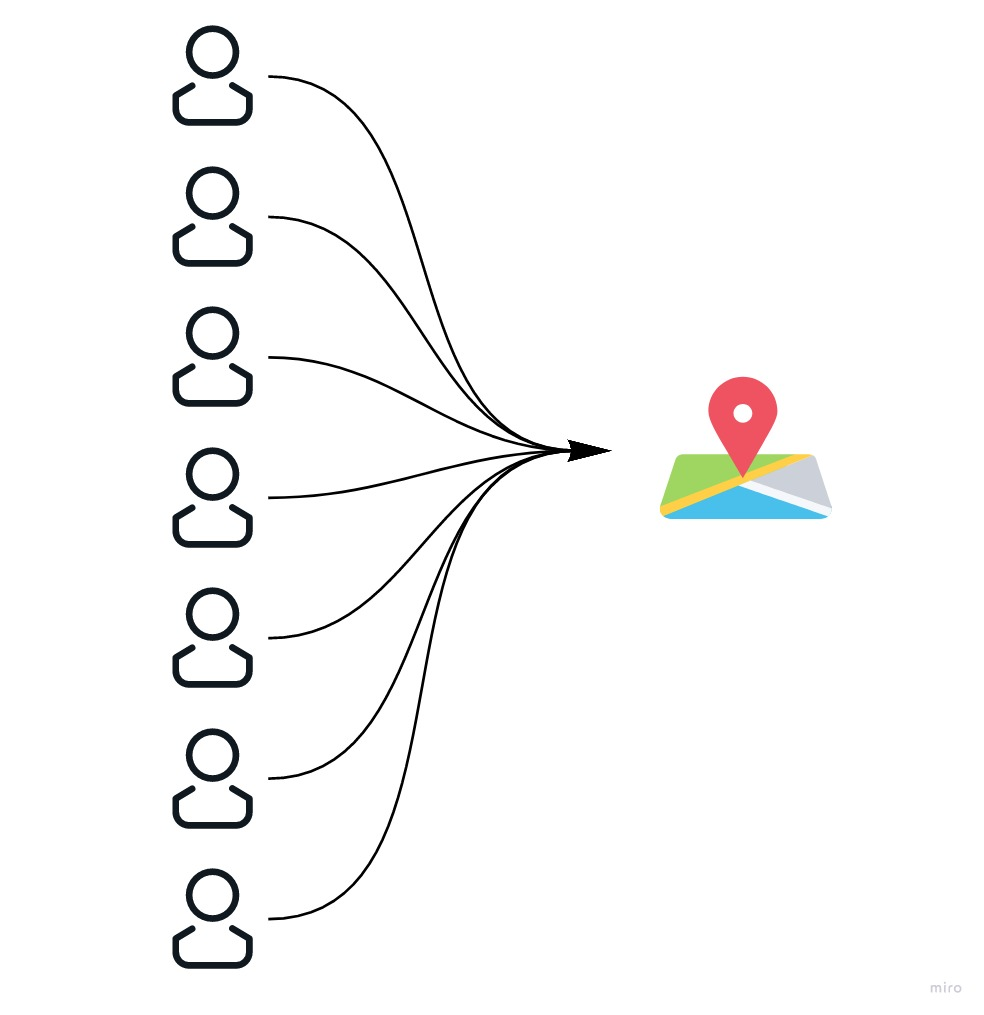
\includegraphics[width=.9\linewidth]{./img/original.jpeg}
\end{center}
\section{MyMaps con Google Forms.}
\label{sec:org4483fe6}
Este es el primer flujo automatizado de información, aquí ya se toma en cuenta el Google Forms y la capa de automatización para el punteo de los incidentes
\begin{center}
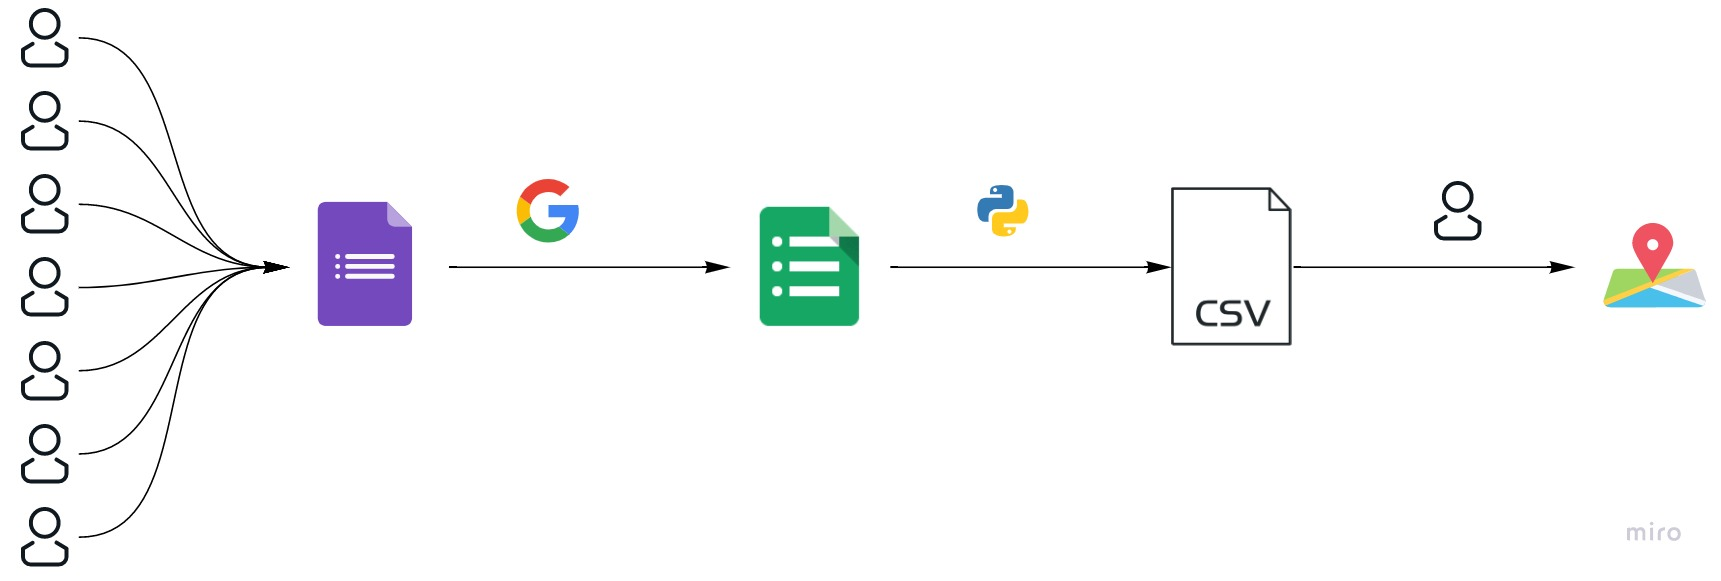
\includegraphics[width=.9\linewidth]{./img/mymaps.jpeg}
\end{center}

\section{CrisisMap}
\label{sec:org7146125}
Se sigue manteniendo la capa de Google Forms para el proceso, sin embargo se usa una capa adicional de Google Big Query que en principio debería conectar automáticamente con Google Crisis Map. Esto no se pudo hacer funcionar, y se tuvo que seguir haciendo la carga manual de los datos.
\begin{center}
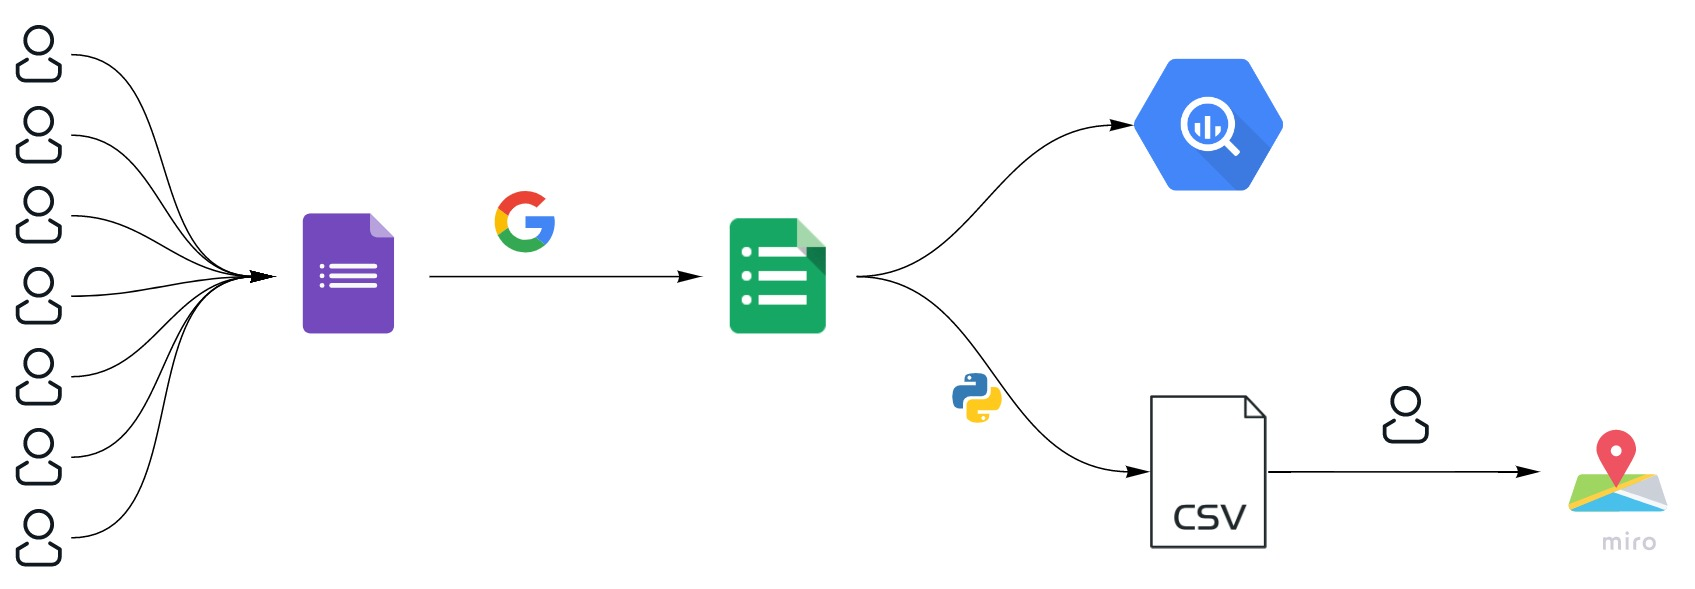
\includegraphics[width=.9\linewidth]{./img/crisismap.jpeg}
\end{center}

\section{Capa de Verificación.}
\label{sec:orgf261fd7}
Esta es un diagrama que ilustra la "Capa de Verificación" que se menciona en el documento, esto hace evidente que habían dos formularios a llenar, uno público y uno más privado para los colaboradores más cercanos
\begin{center}
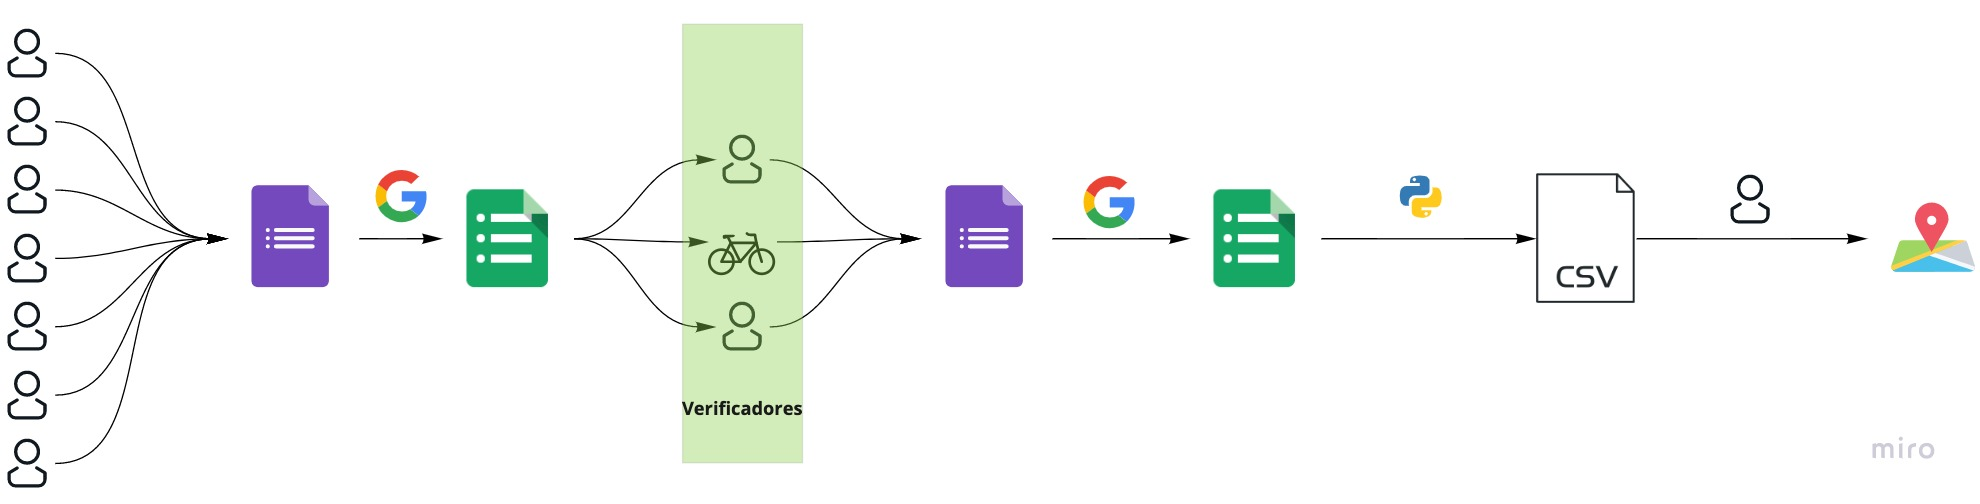
\includegraphics[width=.9\linewidth]{./img/verificacion.jpeg}
\end{center}

\end{appendices}
\end{document}